\section{Schwingkreise}
\subsection{Freie Schwingung}
Die Werte $\textcolor{blue}{U_1,U_2,\beta_u}\text{ sowie
}\textcolor{red}{I_1,I_2,\beta_i}$ müssen aus den Anfangswerten bestimmt
werden.\\
\renewcommand{\arraystretch}{2.3}
\begin{tabular}{| p{4cm} | p{7cm} | p{7cm} |}
	\hline
		& \textbf{Parallelschwingkreis} 
		& \textbf{Serienschwingkreis} \\
	\hline
	& & \\
	& \begin{tikzpicture}[circuit ee IEC, x=2cm, y=2cm, semithick]
	\node (topR) [contact] at (0,1) {};
	\node (bottomR) [contact] at (0,0) {};
	\node at (0,1.2) {};
	
	\draw (topR) to [current direction={very near start, info=$i_R$},
					 resistor={info=R}] (bottomR);
	\draw (topR) -- ++(left:1) 
		to [current direction={very near start, info=$i_L$},
		    inductor={info=L}] ++(down:1)
		-- +(right:1);
	\draw (topR) -- ++(right:1)
		to [current direction={very near start, info=$i_C$},
		    capacitor={info=C}] ++(down:1)
		-- +(left:1);
	\draw[-to, shorten <= 0.2cm,shorten >=0.2cm] (-1.2,1) 
		to node[anchor=east] {$u(t)$} (-1.2,0);
\end{tikzpicture}
	& \begin{circuitikz}[scale=2, european, american inductors]
\ctikzset{bipoles/length=1.2cm}
	\draw
	(0,0)
		to[L=L, o-](1,0)
	(1,0) to[R=R](2,0)
	(2,0) to[C=C, -o](3,0);
\end{circuitikz}


% \begin{tikzpicture}[circuit ee IEC, x=2cm, y=2cm, semithick]
% 	\node (start) [contact] at (0,0) {};
% 	\node (end) [contact] at (3,0) {};
% 	\draw (start) to [inductor={info=L}] (1,0)
% 				  to [resistor={info=R}] (2,0) 
% 				  to [capacitor={info=C}](3,0)
% 				  -- (end);
% 	
% 	\node (placeholder1) at (0,0.5) {};
% 	\node (placeholder2) at (0,-0.5) {};	
% \end{tikzpicture}

% Die Nodes placeholder1 und placeholder2 sind nur dazu da, damit die ganze
% Abbildung wieder gleich hoch ist wie der Parallel-Schwingkreis (siehe
% ParallelSK.tex)
\\
	\hline	
	DGL &
  $\ddot{u} + \dfrac{1}{RC} \dot{u} + \dfrac{1}{LC} u = 0$
  & $\ddot{i} + \dfrac{R}{L} \dot{i} + \dfrac{1}{LC} i = 0$\\
  & $\ddot{u} + \dfrac{\omega_r}{Q_P} \dot{u} + \omega_r^2 u = 0$
  & $\ddot{i} + \dfrac{\omega_r}{Q_S} \dot{i} + \omega_r^2 i = 0$\\
	\hline
	Resonanzfrequenz & \multicolumn{2}{|c|}{$\omega_r =
	\frac{1}{\sqrt{LC}}$} \\
	\hline
	Eigenfrequenz & \multicolumn{2}{|c|}{$\omega_0$} \\
	\hline
	Güte & 
	$Q_P = R\sqrt{\frac{C}{L}} = \frac{R}{\omega_r L}=R\omega_rC$ &
	$Q_S = \frac{1}{R}\sqrt{\frac{L}{C}} = \frac{\omega_r
	L}{R}=\frac{1}{R\omega_rC}$\\
	\hline
	Dämpfungsfaktor & \multicolumn{2}{|c|}{$\xi=\frac{1}{2Q}$} \\
	\hline
	
	Standardstartbedingungen &
	\begin{minipage}{7cm}
    	\vspace{0.1cm}
    	$u(t=0)=U_0$\quad
    	$\dot{u}(t=0)=-\dfrac{U_o}{RC}$ \\
    \end{minipage} &
	\begin{minipage}{7cm}
     	\vspace{0.1cm}
    	$i(t=0)=0$\quad
    	$\dot{i}(t=0)=\dfrac{U_o}{L}$\\   
    \end{minipage}\\
	\hline
	Aperiodisch, $ Q < \frac{1}{2}$
		& $u(t) = \textcolor{blue}{U_1} e^{\alpha_1 t} + \textcolor{blue}{U_2} e^{\alpha_2 t}$ 
		& $i(t) = \textcolor{red}{I_1} e^{\alpha_1 t} + \textcolor{red}{I_2} e^{\alpha_2 t}$ \\
		& $\alpha_{1,2} = - \frac{\omega_r}{2 Q_P} \pm \omega_r \sqrt{\frac{1}{4 Q_P^2} - 1}$	
		& $\alpha_{1,2} = - \frac{\omega_r}{2 Q_S} \pm \omega_r \sqrt{\frac{1}{4Q_S^2} - 1}$\\
		& $U_1 = U_0 \frac{\frac{\omega_r}{Q} +
		\alpha_2}{\alpha_2 - \alpha_1} \quad$ $U_2 = U_0 \frac{\frac{\omega_r}{Q} +
		\alpha_1}{\alpha_1 - \alpha_2}$
		& $I_1 = \frac{U_0}{(\alpha_1 - \alpha_2)L} \quad I_2
		= -I_1$
		\vspace{0.1cm}
		\\
	\hline 	
	Kritisch, $ Q = \frac{1}{2}$
		& $u(t) = (\textcolor{blue}{U_1} + \textcolor{blue}{\beta_u} t) 
		e^{\alpha t} = (\textcolor{blue}{U_1} + \textcolor{blue}{\beta_u} t) 
		e^{- \omega_r t}$ 
		& $i(t) = (\textcolor{red}{I_1} + \textcolor{red}{\beta_i} t) 
		e^{\alpha t} = (\textcolor{red}{I_1} + \textcolor{red}{\beta_i} t) 
		e^{- \omega_r t}$ \\
% 		& $i(t) = \textcolor{red}{I_1} e^{- \omega_r t} +
% 		\textcolor{red}{\beta_i} t e^{- \omega_r t}$ \\ 
		& $\alpha_{1,2} = - \dfrac{\omega_r}{2 Q_P} = - \omega_r$ & 
		$\alpha_{1,2} = - \dfrac{\omega_r}{2 Q_S} = - \omega_r$\\
		& $U_1 = U_0 \quad \beta = -U_0 \left(
		\frac{\omega_r}{Q}+\alpha \right)$ & 
		$I_1 = 0 \quad \beta = \dfrac{U_0}{L}$
		\vspace{0.1cm}
		\\
	\hline 	
	Periodisch, $ Q > \frac{1}{2}$
		& $u(t) = \textcolor{blue}{U_1} e^{\alpha_1 t} + 
					\textcolor{blue}{U_2} e^{\alpha_2 t} $
		& $i(t) = \textcolor{red}{I_1} e^{\alpha_1 t} + 
					\textcolor{red}{I_2} e^{\alpha_2 t} $ \\
	  & $u(t) = e^{-\frac{\omega_r}{2Q_p}t}(U_1\cos(\omega_0 t)+U_2\sin(\omega_0
	  t))$
	  & $i(t) = e^{-\frac{\omega_r}{2Q_s}t}(I_1\cos(\omega_0 t)+I_2\sin(\omega_0
	  t))$\\
% 	 	& $i(t) = \textcolor{red}{I_1} e^{-\frac{\omega_r}{2 Q_S} t} \cos{\omega_0 t} + 
% 					\textcolor{red}{I_2} e^{-\frac{\omega_r}{2 Q_S} t} \sin{\omega_0 t} $ \\
		& $\alpha_{1,2} = - \frac{\omega_r}{2 Q_P} \pm j \omega_r \sqrt{1 - \frac{1}{4 Q_P^2}}$	
		& $\alpha_{1,2} = - \frac{\omega_r}{2 Q_S} \pm j \omega_r \sqrt{1 - \frac{1}{4 Q_S^2}}$	\\
		& $\omega_0 = \omega_r \sqrt{1 - \frac{1}{4 Q_P^2}} \qquad \omega_0 \approx \omega_r (Q_P > 10)$ 
		& $\omega_0 = \omega_r \sqrt{1 - \frac{1}{4 Q_S^2}} \qquad \omega_0 \approx\omega_r (Q_S > 10)$\\
		& $u(t) = \frac{U_0 \omega_r}{\omega_0} e^{- \frac{\omega_r}{2
					Q} t} \cos{[\omega_0 t + \arctan{\frac{1}{\sqrt{4 Q^2 -1}}}]}$
		& $I_1 =  \frac{U_0}{L \cdot 2 \cdot j \omega_0} \quad I_2 = -I_1$
		$ \quad i(t) = \frac{U_0}{\omega_0 L} e^{-\xi  \omega_r  t} \sin{(\omega_0 t)}$
		%%\vspace{0.1cm}
		\\
	\hline
	\end{tabular}
	
\renewcommand{\arraystretch}{\arraystretchOriginal}


\subsection{Erzwungene Schwingung}	


\begin{tabular}{|p{2.4cm}|p{2cm}|p{2cm}|p{2cm}|p{2cm}|p{2cm}|p{2cm}|}
	\hline
		Maximalwerte &
		\multicolumn{3}{|l|}{$I_{Lmax}=I_{Cmax}=\dfrac{I\cdot
   		Q_P}{\sqrt{1-\frac{1}{4Q_P}}}$} &
   	\multicolumn{3}{|l|}{Gilt auch für $U_{Lmax}=U_{Cmax}$ bei
   		dem Serieschwing- } \\
    & \multicolumn{3}{|l|}{$\omega_{I_{Lmax}} =
   		\omega_r\sqrt{1-\frac{1}{2Q_P^2}}\qquad \omega_{I_{Cmax}} =
   		\dfrac{\omega_r}{\sqrt{1-\frac{1}{2Q_P^2}}}$} &
   		\multicolumn{3}{|l|}{kreis, jedoch muss $Q_P$ mit $Q_s$ ersetzt werden.}\\
   \hline
   	Bandbreite, Verstimmung 
   	&
		\multicolumn{3}{|l|}{
			\begin{minipage}[c]{6cm}
			\pgfmathdeclarefunction{gauss}{2}{%
  \pgfmathparse{1/(#2*sqrt(2*pi))*exp(-((x-#1)^2)/(2*#2^2))}%
}

\makebox{\begin{tikzpicture}[scale=0.6, every node/.style={scale=0.6}]
\begin{axis}[
  no markers,
  domain=0:6,
  samples=500,
  hide x axis=true,
	hide y axis=true,
  %height=5cm, width=12cm,
  %xtick={4,6.5}, ytick=\empty,
  enlargelimits=false,
  clip=false,
  axis on top,
  grid = major
  ]
  \addplot {gauss(3,1)};
\end{axis}

	\draw[->, thick] (-0.2,0) -- +(right:7.5) node[right] {$\omega$};
	\draw (2.43,1pt) -- (2.43,-1pt) node[anchor=north] {$\omega_1$};%
	\draw (3.43,1pt) -- (3.43,-1pt) node[anchor=north] {$\omega_r$};%
	\draw (4.43,1pt) -- (4.43,-1pt) node[anchor=north] {$\omega_2$};%

	\draw[->, thick] (0,-0.2) -- +(north:6.5) node[above] {$P$};
	\draw (0.05,3.85) -- (-0.05,3.85) node[anchor=east] {$\frac{Max}{2}$};
	\draw (0.05,5.7) -- (-0.05,5.7) node[anchor=east] {$Max$};

	\draw[->] (1,-0.2) -- +(north:6.5) node[above] {$U/I/Z(\omega)$};
	\draw (1.05,3.85) -- (0.95,3.85) node[anchor=east] {$\frac{Max}{\sqrt{2}}$};
	\draw (1.05,5.7) -- (0.95,5.7) node[anchor=east] {$Max$};

	\draw[dashed] (1,3.85) -- (4.5,3.85);
	\draw[dashed] (1,5.7) -- (3.55,5.7);
	\draw[dashed, shorten <= -3pt] (2.43,4) -- (2.43,0);
	\draw[dashed, shorten <= -3pt] (3.43,5.75) -- (3.43,0);
	\draw[dashed, shorten <= -3pt] (4.43,4) -- (4.43,0);


\end{tikzpicture}}




% \pgfmathdeclarefunction{gauss}{2}{
%   \pgfmathparse{7.5/(#2*sqrt(2*pi))*exp(-((x-#1)^2)/(2*#2^2))}
% }
% 
% \begin{tikzpicture}
% \begin{axis}[every axis plot post/.append style={
% 	 	  mark=none,
% 	 	  domain=0:6,
% 	 	  samples=40,
% 	 	  smooth,
% 	 	  no marks},
% 	 	  hide x axis=true,
% 	 	  hide y axis=true,
% 	 	  enlargelimits=upper]
% 	  \addplot {gauss(0,0.5)};
% 	  \addplot {gauss(3,0.75)};
% 	\end{axis}
% 	\draw[->, very thick] (-0.2,0) -- +(right:6) node[right] {$\omega$};
% 	\draw (2,1pt) -- (2,-1pt) node[anchor=north] {$\omega_1$};
% 	\draw (3,1pt) -- (3,-1pt) node[anchor=north] {$\omega_r$};
% 	\draw (4,1pt) -- (4,-1pt) node[anchor=north] {$\omega_2$};
% 
% 	\draw[->, very thick] (0,-0.2) -- +(north:3.5) node[above] {$P$};
% 	\draw (0.05,2) -- (-0.05,2) node[anchor=east] {$\frac{Max}{2}$};
% 	\draw (0.05,3) -- (-0.05,3) node[anchor=east] {$Max$};
% 
% 	\draw[->] (1,-0.2) -- +(north:3.5) node[above] {$U/I/Z(\omega)$};
% 	\draw (1.05,2) -- (0.95,2) node[anchor=east] {$\frac{Max}{\sqrt{2}}$};
% 	\draw (1.05,3) -- (0.95,3) node[anchor=east] {$Max$};
% 
% 	\draw[dashed] (1,2) -- (4.05,2);
% 	\draw[dashed] (1,3) -- (3.05,3);
% 	\draw[dashed, shorten <= -3pt] (2,2) -- (2,0);
% 	\draw[dashed, shorten <= -3pt] (3,3) -- (3,0);
% 	\draw[dashed, shorten <= -3pt] (4,2) -- (4,0);
% 
% \end{tikzpicture}




% \pgfmathdeclarefunction{gauss}{2}{
%   \pgfmathparse{1/(#2*sqrt(2*pi))*exp(-((x-#1)^2)/(2*#2^2))}
% }

% \begin{tikzpicture}
% 	\begin{axis}[every axis plot post/.append style={
% 	  mark=none,
% 	  domain=0:6,
% 	  samples=10,
% 	  smooth, % All plots: from -2:2, 50 samples,
% 	  no marks},
% 	  hide x axis=true, % no box around the plot, only x and y axis
% 	  hide y axis=true, % the * suppresses the arrow tips
% 	  enlargelimits=upper] % extend the axes a bit to the right and top
% 	\addplot {gauss(3,0.75)}
%   
%   \end{axis}
%   
% 	\draw[->, very thick] (-0.2,0) -- +(right:6) node[right] {$\omega$};
% 	\draw (2,1pt) -- (2,-1pt) node[anchor=north] {$\omega_1$};
% 	\draw (3,1pt) -- (3,-1pt) node[anchor=north] {$\omega_r$};
% 	\draw (4,1pt) -- (4,-1pt) node[anchor=north] {$\omega_2$};
% 
% 	\draw[->, very thick] (0,-0.2) -- +(north:3.5) node[above] {$P$};
% 	\draw (0.05,2) -- (-0.05,2) node[anchor=east] {$\frac{Max}{2}$};
% 	\draw (0.05,3) -- (-0.05,3) node[anchor=east] {$Max$};
% 
% 	\draw[->] (1,-0.2) -- +(north:3.5) node[above] {$U/I/Z(\omega)$};
% 	\draw (1.05,2) -- (0.95,2) node[anchor=east] {$\frac{Max}{\sqrt{2}}$};
% 	\draw (1.05,3) -- (0.95,3) node[anchor=east] {$Max$};
% 
% 	\draw[dashed] (1,2) -- (4.05,2);
% 	\draw[dashed] (1,3) -- (3.05,3);
% 	\draw[dashed, shorten <= -3pt] (2,2) -- (2,0);
% 	\draw[dashed, shorten <= -3pt] (3,3) -- (3,0);
% 	\draw[dashed, shorten <= -3pt] (4,2) -- (4,0);
%   
%   
% \end{tikzpicture}



% \begin{tikzpicture}
% \begin{axis}[every axis plot post/.append style={
% 	mark=none,domain=0:6,samples=50,smooth},
% 	hide x axis=true,
%   hide y axis=true
%   ]

%	\draw[->, very thick] (-0.2,0) -- +(right:6) node[right] {$\omega$};
%	\draw (2,1pt) -- (2,-1pt) node[anchor=north] {$\omega_1$};
% 	\draw (3,1pt) -- (3,-1pt) node[anchor=north] {$\omega_r$};
% 	\draw (4,1pt) -- (4,-1pt) node[anchor=north] {$\omega_2$};
% 	
% 	\draw[->, very thick] (0,-0.2) -- +(north:3.5) node[above] {$P$};
% 	\draw (0.05,2) -- (-0.05,2) node[anchor=east] {$\frac{Max}{2}$};
% 	\draw (0.05,3) -- (-0.05,3) node[anchor=east] {$Max$};
% 	
% 	\draw[->] (1,-0.2) -- +(north:3.5) node[above] {$U/I/Z(\omega)$};
% 	\draw (1.05,2) -- (0.95,2) node[anchor=east] {$\frac{Max}{\sqrt{2}}$};
% 	\draw (1.05,3) -- (0.95,3) node[anchor=east] {$Max$};
% 	
% 	\draw[dashed] (1,2) -- (4.05,2);
% 	\draw[dashed] (1,3) -- (3.05,3);
% 	\draw[dashed, shorten <= -3pt] (2,2) -- (2,0);
% 	\draw[dashed, shorten <= -3pt] (3,3) -- (3,0);
% 	\draw[dashed, shorten <= -3pt] (4,2) -- (4,0);

  
% 	\addplot {gauss(1,0.75)}
% 
% \end{axis}
% \end{tikzpicture}
			\end{minipage}} &
		\multicolumn{3}{|l|}{
			\begin{minipage}[c]{6cm}
  			$b_w = \omega_2 - \omega_1 = \dfrac{\omega_r}{Q}$\\
  			$B = \dfrac{f_r}{Q}=\dfrac{b_w}{2\pi}$\\\\
				$\eta = \dfrac{\omega}{\omega_r} - \dfrac{\omega_r}{\omega} \qquad
				\dfrac{Z}{R} = \dfrac{U}{U_{max}} = \dfrac{1}{\sqrt{1 + (\eta Q)^2}}$
			\end{minipage}}\\
	\hline
		& \multicolumn{2}{|l|}{$\omega = \omega_1$}
		& \multicolumn{2}{|l|}{$\omega = \omega_r$}
		& \multicolumn{2}{|l|}{$\omega = \omega_2$} \\
	\hline
		Zeigerdiagramme &
		\multicolumn{2}{|l|}{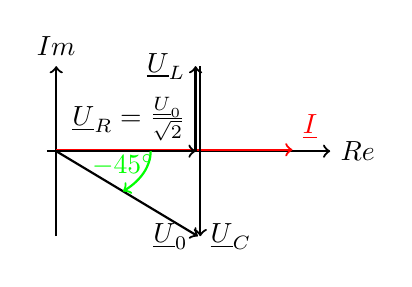
\begin{tikzpicture}[scale=0.6, yscale=0.6, thick]
	%Koordinatensystem
	\draw[->] (-0.2,0) -- +(right:6) node[right] {$Re$};
	\draw[->] (0,-3) -- +(north:6) node[above] {$Im$};
	
	%Pfeile
	\draw[->, color=red] (0,0.05) -- +(right:5) node[above right]
	{$\underline{I}$};
	\draw[->] (0,0) -- +(right:2.95) node[above left] {$\underline{U}_R
	= \frac{\underline{U}_0}{\sqrt{2}}$};
	\draw[->] (2.95,0) -- (2.95,3) node[left]
	{$\underline{U}_L$};
	\draw[->]	(3.05,3) -- (3.05,-3) node[right] {$\underline{U}_C$};
	\draw[->] (0,0) -- (3,-3) node[left] {$\underline{U}_0$};
	
	%Winkel
	\draw[->, color = green] (2,0) arc (0:-45:2) node[above = 2]
	{$-45^{\circ}$};

\end{tikzpicture}


} &
		\multicolumn{2}{|l|}{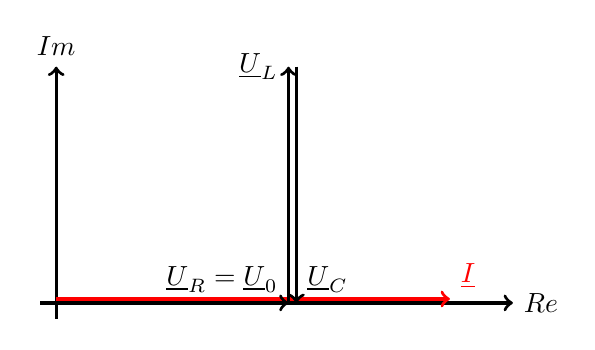
\begin{tikzpicture}
	%Koordinatensystem
	\draw[->, very thick] (-0.2,0) -- +(right:6) node[right] {$Re$};
	\draw[->, very thick] (0,-0.2) -- +(north:3.2) node[above] {$Im$};
	
	%Pfeile
	\draw[->, color=red, very thick] (0,0.05) -- +(right:5) node[above right]
	{$\underline{I}$};
	\draw[->, very thick] (0,0) -- +(right:2.95) node[above left] {$\underline{U}_R
	= \underline{U}_0$};
	\draw[->, very thick] (2.95,0) -- (2.95,3) node[left]
	{$\underline{U}_L$};
	\draw[->, very thick]	(3.05,3) -- (3.05,0) node[above right]
	{$\underline{U}_C$};

\end{tikzpicture}

} &
		\multicolumn{2}{|l|}{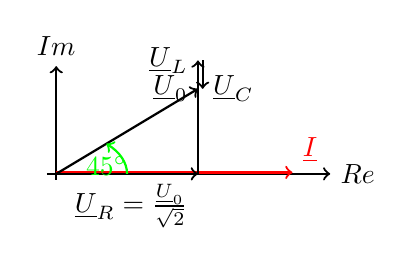
\begin{tikzpicture}[scale=0.6, yscale=0.6, thick]
	%Koordinatensystem
	\draw[->] (-0.2,0) -- +(right:6) node[right] {$Re$};
	\draw[->] (0,-0.2) -- +(north:4) node[above] {$Im$};
	
	%Pfeile
	\draw[->, color=red] (0,0.05) -- +(right:5) node[above right]
	{$\underline{I}$};
	\draw[->] (0,0) -- +(right:3) node[below left] {$\underline{U}_R
	= \frac{\underline{U}_0}{\sqrt{2}}$};
	\draw[->] (3,0) -- (3,4) node[left]
	{$\underline{U}_L$};
	\draw[->]	(3.10,4) -- (3.10,3) node[right] {$\underline{U}_C$};
	\draw[->] (0,0) -- (3,3) node[left] {$\underline{U}_0$};
	
	%Winkel
	\draw[->, color = green] (1.5,0) arc (0:45:1.5) node[below = 1]
	{$45^{\circ}$};

\end{tikzpicture}


} \\
	\hline
\end{tabular}

\renewcommand{\arraystretch}{\arraystretchOriginal}

\subsection{Verlustbehafteter Schwingkreis}
Resonanzfrequenz $\omega_r$ tritt dort auf, wo 
$\operatorname{Im} \{ \underline{Y}(\omega) \} =
\operatorname{Im}\{\underline{Z}(\omega) \} = 0$.

\subsection{Resonanzkreis mit realen Elementen}
Umrechnungen Parallel- $\Longleftrightarrow$ Serieschaltungen von L \& R oder C \& R. \\

% Siehe http://www.causa-dura.ch/Scripts/aet\_skript.pdf, seite 121 
\renewcommand{\arraystretch}{1.1}
\begin{tabular}{| p{2cm} | p{8cm} | p{8cm} |}
	\hline
		& \textbf{Parallel $\Rightarrow$ Seriell}  
		& \textbf{Seriell $\Rightarrow$ Parallel} \\
	\hline
		L \& R
		& $ R_S = \dfrac{R_P (\omega L_P)^2}{R_P^2 + (\omega L_P)^2} \qquad 
			L_S = \dfrac{R_P^2 L_P}{R_P^2 + (\omega L_P)^2}  $
		& $ R_P = \dfrac{R_S^2 + (\omega L_S)^2}{R_S} \qquad 
			L_P = \dfrac{R_S^2 + (\omega L_S)^2}{\omega^2 L_S}   $ \\
	\hline	
		C \& R
		& $ R_S = \dfrac{R_P}{1 + (\omega R_P C_P)^2} \qquad 
			C_S = \dfrac{1 + (\omega R_P C_P)^2}{(\omega R_P)^2 C_P}$
		& $ R_P = \dfrac{(\omega C_S R_S)^2 + 1}{(\omega C_S)^2 R_S} \qquad
			C_P = \dfrac{C_S}{1 + (\omega C_S R_S)^2}$\\
	\hline
\end{tabular}
\renewcommand{\arraystretch}{1}
